\documentclass[a4paper]{report}

\usepackage{masterThesisEn}
\usepackage{graphicx}
\usepackage{xspace}
\usepackage{multirow}
\usepackage{url}
% [required] Title:\maintatile{title}
\maintitle{A Study on Time Series Topic Popularity Extraction Methods with Topic Modeling}

% [required] Published date:\publish{year}{month}
\publish{2020}{September}

% [required] Student ID:\student{ID number}{Name}
\student{201826098}{Khan, Muhammad Haseeb UR Rehman}

% [required] Abstract:\abst{abstract}
\abst{Understanding large document datasets is a fundamental natural language processing (NLP) problem.
A large document collection is often generated as an accumulation for a long time span, which naturally has a time series structure.
One of the important aspects of understanding such document collection is an estimation of time series topic popularity, which means the amount of mention of topics in each time slice.
Topic modeling is an unsupervised NLP technique that constructs a set of topics pervaded in a given document dataset by a grouping process like a clustering.
Particularly for modeling time series documents, Dynamic Topic Model (DTM) has been proposed to capture dynamic changes of topics over time.
DTM is considered to be suitable to model time series documents since the basic topic model called Latent Dirichlet Allocation (LDA) assumes a static set of topics.

However, DTM has a drawback that is a high computation cost, whereas LDA is far faster thanks to its simplicity in the model architecture.
For this reason, people have a motivation to employ LDA rather than DTM even for time series document collections.
The collections of topics extracted by DTM and LDA are different, but little insight has been known about how they are different in practice.

In this paper, we extensively compare the topics extracted by LDA for time series document collections with the topics induced by DTM through a new objective analysis.
Topic drifting and popularity are two fundamental aspects of time series topic analysis. 
We conducted experiments with multiple datasets to check the reliability of the information extracted from both models. 
We used Jensen-Shannon (JS) similarity-based analysis to check for information overlap, also overall and time series correlation analysis as an inverse approach to extract DTM information from LDA topics. 
Lastly, we constructed time series topic popularity graphs for both models from the document-topic distributions and compared the results. 
Our results show that there is notable DTM topic drifting information in some cases and sometimes no or vague topic drifting. 
Topic drifting embedded in DTM topics makes this model less favorable for topic popularity analysis. 
On the other hand, LDA topics with no time transition information provided concrete results of topic popularity. 
Thus, for time series topic popularity analysis, LDA is the accurate choice from both models.
}

% [required] Academic advisors:\advisors{Principal}{Secondary}
\advisors{Kei Wakabayashi}{Atsuyuki Morishima}


% output
\begin{document}

\makecover

\addtolength{\textheight}{-5mm}
\setlength{\footskip}{15mm}	% set footer
% List of contents/figures

\justifying

%\addtolength{\topmargin}{-20mm}

\fontsize{11pt}{15pt}\selectfont

\pagebreak\setcounter{page}{1}
\pagenumbering{roman} % I, II, III, IV 
\pagestyle{plain}
\tableofcontents
\listoffigures

% contents
\parindent=2em	% set indent
\pagebreak\setcounter{page}{1}
\pagenumbering{arabic} % 1,2,3
\pagestyle{plain}

%%%%%%%%%%%%%%%%%%%%%%%%%%%%%%%%%%%%%%%%%%%%%%%%%%%%%%%%%

\chapter{Introduction}
Natural language processing addresses the task of understanding texts through language modeling, information extraction, summarization and classification among others. 
Large document datasets often involve time series document collections, such as Twitter posts, news articles, and academic paper archives, because a continuous accumulation of documents typically yields a massive amount of text data. 
By focusing on the nature of time series, many useful applications can be developed, such as bursty topic detection \cite{koike2013time}, trend analysis \cite{kawamae2011trend,zhang2015market}, topic evolution analysis \cite{kalyanam2015context,xie2016topicsketch}, topic transition pattern mining \cite{kim2015toptrak} and more. 
All above mentioned applications are related to topic modeling which is an unsupervised way of finding a set of topics by grouping and estimating process similar to clustering.
Latent Dirichlet Allocation (LDA) \cite{blei2003latent} and Dynamic Topic Model (DTM) \cite{blei2006dynamic} are widely used topic models that revolutionized the solving of unsupervised topic modeling-based NLP problems.

To capture the time series features of topics, DTM and its related-models \cite{amoualian2016streaming,acharya2018dmdtm} assume dynamic drift of distributions, whereas in LDA a static set of topics are drawn by ignoring the time series information of documents in training process.
Although the DTM-based models appropriately find topics over time, they require expensive computational cost, which can be a critical drawback in some applications.
On the other hand, there is a large body of work developing efficient inference algorithms for LDA \cite{yut2017lda,chen2018scalable,yuan2015lightlda,chen2015warplda,yu2015scalable} because of its simpler architecture compared to DTM.
While both models learn and work differently and even give different results, some practitioners and researchers employ LDA instead to analyze the time series nature to take advantage of its efficiency.

The question that arises in this background is; if time series topics information can be extracted by using LDA, which is faster than DTM, then why do we need to use DTM?
To answer the above-mentioned question this research was conducted with a problem statement ``\emph{Can time series topic information of DTM be extracted from LDA?}''.
To the best of our knowledge, there have been no studies that extensively compared the information extracted using LDA with that of DTM.

In this research, we examined the differences between LDA topics and DTM topics by using multiple datasets and model configurations.
For this, we had to compare two sets of topics from both models. Topic drifting and topic popularity are fundamental time series information that can be extracted from DTM. Topic drifting is the topic transition over time and popularity is the measure of topic proportion at each time slice. The challenging part in topic transition analysis is that DTM topic set has a sequential structure whereas LDA topic set has no sequential type of information. To map the unstructured topic set with DTM topics, we used a probability distribution similarity method.

Based on this matching, we analyzed both topic sets and in this process, we encountered with fragmentation issue, which is explained in detail in Chapter 4 (Figure \ref{fig:fragmentation}).
DTM provides the time evaluation of topics, which means one single DTM topic can shift to a new subject if compared with the initial time's topic subject, whereas a LDA topic's theme remains the same because LDA has no time aspect. This shift in DTM topics when compared and confirmed with LDA topics is called fragmentation. In this experiment, we found that some DTM topics contain information on two or more LDA topics; in other words, they have two or more fragmented topics.

To extract topics drifting from LDA topics, we compared both models by trying different approaches including correlation analysis and time series topic correlation. For topic popularity analysis, the problem is LDA doesn't model variation of topics so we had to find a way to see the topics variation in time series manner to compare it with DTM topics. Therefore, we experimented and introduced a way to transform LDA generated topics to time series trend analysis that is explained in detail in Chapter 3. We built time series population graphs for the topics of both models. Because both models have different types of information, there are pros and cons for each model. LDA extracts the focus on the collection of topics, whereas DTM can find connections between different themes and how subjects interchange within the same domain or topic.

Even though DTM has the edge of finding topic transitions over time for time series data, in most cases, constructing only population graphs for LDA topics is enough for time series analysis \cite{aubert2013clustering,pan2011event,shirota2014extraction}.
Some specific problems in which topic transition extraction is mandatory requires DTM despite its high computation cost (e.g., determining the focuses and trends of protected technological innovations across the entire disease landscape \cite{huang2019technological}).In this paper, we provide empirical evidence that demonstrates these practical insights based on the extensive experiment.

%%%%%%%%%%%%%%%%%%%%%%%%%%%%%%%%%%%%%%%%%%%%%%%%%%%%%%%%%%%%

\chapter{Related Work}
Koike et al. \cite{koike2013time} proposed a method that draws a time series graph to find the bursty topic detection in Twitter data individually, as well as with correlated news, by using DTM \cite{blei2006dynamic}. They applied DTM to extract 50 topics from a subset of news articles and Twitter about \textit{``The London Olympics''}. For Twitter dataset, it is believed that there are many diverse topics including almost anything people talk in their lives ranging from personal \emph{(My cat is weird)}, sentimental \emph{(Today, I am very happy because I finished my work early)}, political \emph{(USA is banning Chinese products)}, and much more. So, if someone truly needs to analyze tweet's data without any preprocessing keyword selection then the number of topics selection should be way higher. Even though DTM allows the distribution of topics and words to be changed over time, DTM has a drawback in the computational cost, which particularly prevents to increase the number of topics $K$ to hundreds or thousands. 

For topic modeling problems, the most popular topic model used in the research community is LDA \cite{blei2003latent}. Even though LDA doesn't provide the topic transition over time but topic-word distributions and document-topic distributions can be extracted. With these distributions along with time series information of documents, topic distribution graphs can be built in time series fashion. Theoretically, Koike et al.'s research can be performed by using LDA as a topic model. So the question arises, why do we need DTM that has very high computation cost when we can use LDA. This question is the baseline of this research.

To understand this research better, we had to start from the basics which are algorithms of both topic models. The main generative process of LDA with parameters $\alpha$ and $\beta$ is explained below and the implicit assumption is that, documents are drawn interchangeably from the same set of topics.
\begin{enumerate}
\item For each document:
\begin{enumerate}
\item  Draw $\theta \sim Dir(\alpha)$
\item For each word:
\begin{enumerate}
\item Draw $ Z \sim Mult (\theta) $
\item Draw $ W_{d, n} \sim Mult(\beta_z)$
\end{enumerate}
\end{enumerate}
\end{enumerate}

The logistic normal with mean $ \alpha $ to express uncertainty over proportions is part of DTM rather than the topic proportions $\theta$ drawn from Dirichlet distribution. Thus, DTM's generative process for slice $t$ of the sequential corpus is:

\begin{enumerate}
\item Draw topics $ \beta_t | \beta_{t-1}  \sim N(\beta_{t-1}, \sigma^2I) $
\item Draw $ \alpha_t | \alpha_{t-1}  \sim N(\alpha_{t-1}, \delta^2I) $
\item For each document:
\begin{enumerate}
\item Draw $ \eta \sim N(\alpha_t, a^2I)$
\item For each word:
\begin{enumerate}
\item Draw $Z \sim Mult(\pi(\eta)) $
\item Draw $W_{t,d,n} \sim Mult(\pi(\beta_{t,z})) $
\end{enumerate}
\end{enumerate}
\end{enumerate}

$\pi$ is a mapping factor that maps the multinomial natural parameters to the mean parameters, $\pi(\beta_{k, t})_w = \frac{exp(\beta_{k,t,w})}{\sum_{w'} exp(\beta_k,t,w')}$. For a detailed explanation, please refer to the following papers: LDA \cite{blei2003latent} and DTM \cite{blei2006dynamic}. 
\begin{figure}[ht!]
    \begin{tabular}{cc}
    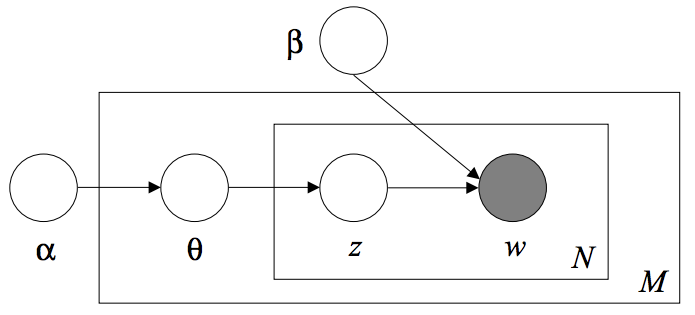
\includegraphics[scale=0.6]{lda_generative}
    & 
    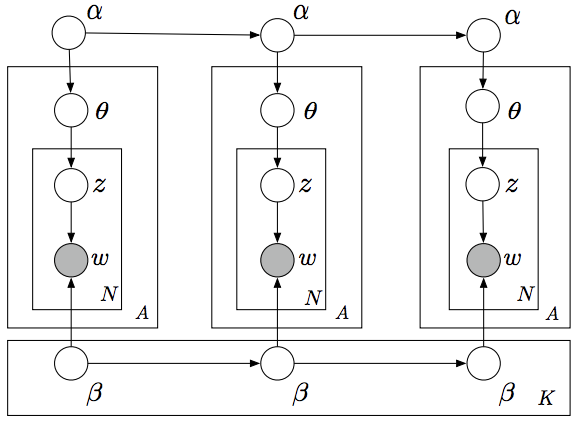
\includegraphics[scale=0.6]{dtm_generative}
    \end{tabular}
\caption{Graphical model representations of LDA (left) and DTM (right) are shown here from the original papers \cite{blei2003latent, blei2006dynamic}. In LDA, outer box (M) represents documents, while the inner plate (N) represents repeated choice of topics and words with documents. In DTM, box (A) represents documents, box (N) is same as LDA and $\alpha$ \& $\beta$ evolve over time.}
\label{fig:graphical_model_representation}
\end{figure}

From the above mentioned generative processes and graphical model representations (Figure \ref{fig:graphical_model_representation}) of both models, we can observe that random variable $\alpha$ and $\beta$ appear only once in LDA whereas in DTM we have these random variables with each time slice.
The number of latent random variables to be estimated considerably affects the computational complexity of training algorithms \cite{li2014reducing, yao2009efficient}. In this paper, we empirically compare the computation time of the algorithms in Chapter 6.

Before applying topic modeling, some preprocessing steps are required because documents are messy and can provide poor results when topic models are applied. Applying linguistic preprocessing may be of some help \cite{han2012automatically}. Topic models perform pretty well with long document datasets (e.g., News articles) but topic models don't perform well on short text documents (e.g., Twitter) so tweet pooling is used for making relatively big documents for the Twitter dataset. Tweet pooling has been proposed, and later proved experimentally \cite{mehrotra2013improving}, as an intuitive solution \cite{hong2010empirical,zhao2011comparing} when models perform poorly with a tweets dataset because of small document size.

Hashtag pooling outperformed all other pooling schemes \cite{mehrotra2013improving} and it is making documents based on hashtags where all the tweets with one hashtag form a single document. Any tweet having more than one hashtag is added to the tweet pool of each of those hashtags. A new, under-examined hashtag pooling proposed as day-hashtag pooling was used in the inference part of Twitter dataset analysis.
Day-hashtag pooling is a combination of hashtag pooling and temporal pooling proposed by Mehrotra et al. \cite{mehrotra2013improving} and even though the author showed a possibility of hashtag-time pooling scheme but it is almost ignored in past. All the tweets with one hashtag on a specific date are grouped to make a single document.

%%%%%%%%%%%%%%%%%%%%%%%%%%%%%%%%%%%%%%%%%%%%%%%%%%%%%%%%%%%

\chapter{Time Series Topic Estimation by LDA}
LDA topics information is organized by time to compare it with DTM topics. LDA assumes a latent topic distribution for each document $d$ denoted by $\theta_{d}$ and a latent topic assignment $z_i$ for each word $w_i$ in a document.
The word $w_i \in W$ is drawn from a distribution of words associated to the assigned topic $z_i = k$, which is denoted by $\phi_{k}$.
We trained the LDA with multiple datasets without any modification to the LDA machinery.
Formally, when we denote a set of documents that we would like to analyze by $X = \{\mathbf{x}_1, \dots, \mathbf{x}_D\}$, we simply use $X$ as a training dataset for ordinary LDA training.
Before the LDA training, we apply a pooling method when we deal with a short text dataset such as Twitter.
In that case, each document $\mathbf{x}_d$ consists of multiple text instances (e.g., tweets).
We denote the number of instances that are contained in a document $\mathbf{x}_d$ by $T_d$.
If no pooling method is applied, $T_d = 1$ for all documents.

For the inference part that estimates the number of documents for each topic, we take the time information into account.
Each document $\mathbf{x}_d$ is associated to a specific time slice, which we denote by $\tau(\mathbf{x}_d)$.
Let $X_t = \{ \mathbf{x} \in X | \tau(\mathbf{x}) =  t \}$ be a set of documents in time slice $t$.
We estimate the topic distribution $\theta_{d}$ for each document in $X$ and calculate the estimated number of documents for each topic $k$ at each time slice $t$, denoted by $N_k^t$, using the following equations:

\begin{equation}
N_k^t = \sum_{d: \mathbf{x}_d \in X_t} \theta_{dk}  T_d
\label{eq:N_k_t}
\end{equation} 

Probability distribution $\mathbf{\theta}_d$ is calculated using Dirichlet distribution by applying LDA to the input data. Given words $ \mathbf{x}_d = w_1, \dots , w_M$ we estimate the distribution of $\theta_d$.
\begin{equation}
p(\theta_d|\mathbf{x}_d) = \sum_\mathbf{z} p(\theta_d|\mathbf{z})p(\mathbf{z}|\mathbf{x}_d)
\end{equation}
Where corresponding topics $\mathbf{z} = z_1, \dots, z_K$ and the summation is over all possible assignments of $\mathbf{z}$. Since summation is analytically intractable, we apply Monte Carlo approximation with only one sample. We obtain a sample $ \hat{\mathbf{z}} $ from $ p(\mathbf{z}|\mathbf{x}_d) $ using (collapsed) Gibbs sampling with five iterations. This approximation reduces the equation into the posterior probability of $ \theta_d $ given $ \hat{\mathbf{z}} \sim p(\mathbf{z}|\mathbf{x}_d) $.
\begin{equation}
p(\theta_d|\mathbf{x}_d) \approx p(\theta_d|\hat{\mathbf{z}})
\end{equation}
The posterior is a Dirichlet distribution of which the expectation $\hat{\theta}_d$ is:
\begin{equation}
\hat{\theta}_{dk} = \frac{n_k + \alpha_k}{N + \sum_{k'} \alpha_{k'}}
\end{equation}
where $ n_k = \sum_{i=1}^N \delta(\hat{z_i}, k) $, i.e., the number of topic k in $\hat{\mathbf{z}}$.

The final step is to estimate the number of documents to make the time series popularity graphs. By using $\hat{\theta}_{dk}$, we calculate the $N_k^t$ using Equation (\ref{eq:N_k_t}). Since $N_k^t$ is the estimated number of documents for topic $k$ at time slice $t$, we can draw the time series popularity for topic $k$ by plotting $(t, N_k^t)$ on a plain.

%%%%%%%%%%%%%%%%%%%%%%%%%%%%%%%%%%%%%%%%%%%%%%%%%%%%%%%%%%

\chapter{Similarity Analysis of DTM and LDA Topics}
The topics we get from both DTM and LDA are in the form of distributions. Along with the top words we also get the probability of occurrence of each word. An example of word distribution of a topic is shown in Table \ref{table:topicDistribution}, where the first element of the tuple is a word and the second element is the probability of this word in the current topic. We extract the top 50 words for all the topics so word distribution is represented by $K \times 50$ matrix in LDA and $K$ is the number of topics. Top 50 words are enough to convey the meaning of the topic and probability density for lower ranked words is very low and doesn't effect much in topic-word probability distributions. The top words may change in a DTM topic over time, so overall word distribution of a DTM topic varies, but it is 50-dimensional vector for one time slice, the same as a LDA topic. To check the relation between a DTM topic and a LDA topic, we use a simple but widely accepted similarity measure, the Jensen-Shannon (JS) divergence \cite{lin1991divergence}. Only the top 50 words are considered for this similarity measure and word distributions do not sum up to one, so we apply normalization on both the DTM and LDA topic-word distributions. 
We denote the normalized top 50 word distribution for the $k$th LDA topic by $\tilde{\phi}_{k}$ and for $j$th DTM topic at time slice $t$ by $\tilde{\phi}_j^t$. Each distribution $\phi$ is a $|W|$-dimensional vector that represents the parameter of a categorical distribution of words where $W$ is a set of the vocabulary. 
The JS divergence between these distributions is defined as:

\begin{equation}
JSD(\tilde{\phi}_k || \tilde{\phi}_j^t) = \frac{1}{2} D_{KL}(\tilde{\phi}_k || T_{M}) + \frac{1}{2} D_{KL}(\tilde{\phi}_j^t || T_{M})
\label{eq:jsd}
 \end{equation}
 where
 \begin{equation}
  T_M = \frac{1}{2}(\tilde{\phi}_k + \tilde{\phi}_j^t)
 \end{equation}
 $D_{KL}(\phi_1 || \phi_2)$ is the Kullback-Leibler divergence and can be calculated by below mentioned equation:
 \begin{equation}
D_{KL}(\phi_1 || \phi_2)  =  \sum_{w \in W} P(w| \phi_1) \log \frac{P(w| \phi_1)}{P(w| \phi_2)}
 \end{equation}
%  \begin{equation}
% D_{KL}(\tilde{\phi}_k || \tilde{\phi}_j^t)  =  \sum_{w \in W} P(w| \tilde{\phi}_k) \log \left( \frac{P(w| \tilde{\phi}_k)}{P(w| \tilde{\phi}_j^t)} \right)
%  \end{equation}

\begin{table}[ht!]
\begin{tabular}{|p{1cm}|p{13cm}|}
\hline \textbf{DTM}  &
('space', 0.0904)	('dimensional', 0.0492)	('nearest', 0.0346)	('data', 0.0341)	('projection', 0.0256)	('local', 0.0226)	('vectors', 0.0211)	('mapping', 0.0209)	('neighbor', 0.0159)	('maps', 0.0144)	('tangent', 0.0138)	('neighborhood', 0.0131)	('dimensions', 0.0125)	('dimension', 0.0122)	('dimensionality', 0.0122)	('feature', 0.0122)	('neighbors', 0.0114)	('points', 0.0097)	('kernel', 0.0091)	('point', 0.0091)	('coordinates', 0.0091)	('transformation', 0.0083)	('quantization', 0.0076)	('euclidean', 0.0074)	('projections', 0.0064)	('locally', 0.0064)	('manifold', 0.0062)	('structure', 0.0062)	('distances', 0.0059)	('reduction', 0.005)	('onto', 0.0048)	('spaces', 0.0048)	('nonlinear', 0.0044)	('topology', 0.0042)	('topological', 0.004)	('subspace', 0.004)	('directions', 0.0039)	('invariant', 0.0037)	('product', 0.0037)	('knn', 0.0036)	('coordinate', 0.0035)	('closest', 0.0034)	('matrix', 0.0031)	('mapped', 0.003)	('principal', 0.003)	('two', 0.003)	('multidimensional', 0.0029)	('laplacian', 0.0027)	('rbf', 0.0025)	('rotation', 0.0024) \\ \hline

\textbf{LDA} &
('inference', 0.034)	('map', 0.025)	('belief', 0.018)	('propagation', 0.018)	('message', 0.014)	('approximate', 0.012)	('product', 0.011)	('exact', 0.011)	('energy', 0.011)	('constraints', 0.01)	('partition', 0.01)	('marginal', 0.01)	('graphical', 0.01)	('sum', 0.009)	('probabilistic', 0.009)	('program', 0.008)	('assignment', 0.008)	('messages', 0.008)	('passing', 0.008)	('marginals', 0.008)	('field', 0.007)	('factor', 0.007)	('evidence', 0.007)	('potentials', 0.007)	('markov', 0.006)	('domain', 0.006)	('pairwise', 0.006)	('free', 0.005)	('factors', 0.005)	('potential', 0.005)	('fields', 0.005)	('mrf', 0.005)	('crf', 0.005)	('loopy', 0.005)	('approximations', 0.004)	('discrete', 0.004)	('constraint', 0.004)	('intelligence', 0.004)	('tractable', 0.004)	('ground', 0.004)	('ising', 0.004)	('lifted', 0.004)	('formula', 0.003)	('artificial', 0.003)	('logic', 0.003)	('weight', 0.003)	('configuration', 0.003)	('complexity', 0.003)	('represent', 0.003)	('original', 0.003) \\ \hline

\end{tabular}
\caption{Topic-word distribution of sample DTM and LDA topics}
\label{table:topicDistribution}
\end{table}

\section{Matching DTM and LDA Topics}
JS analysis tells us about the information overlap between DTM and LDA topics and is a good way to confirm weather the topics are similar in both models or that the topic-word distributions are totally different. This analysis also illustrates fragmentation of topics that is explained below in detail. The JS similarity measure changes between two or more LDA topics and a DTM topic over time. An example is shown in Figure \ref{fig:fragmentation}, where we see that the sample DTM topic was ``Tensor decomposition for signal processing'' in the starting years, but from 2005 onward the topic's theme shifted rapidly towards ``Tensor decomposition'' and ``Signal processing'' was no longer significant. Whereas ``Tensor decomposition'' and ``Signal Processing'' are two different topics found in LDA analysis. We call this fragmentation phenomenon because the topic is recognized as a single drifting topic by DTM but LDA splits it into two or more topics. By subjective analysis, JS value of 0.7 is selected as threshold value for fragmented topics analysis.

Formally, we say the $j$th DTM topic is \textit{related} to the $k$th LDA topic if there exists $t$ such that $JSD(\tilde{\phi}_k || \tilde{\phi}_j^t) \leq 0.7$.
We say the $k$th and $l$th LDA topics are fragmented topics of the $j$th DTM topic if the $j$th DTM topic is related to both the $k$th and $l$th LDA topics.

\begin{figure*}[t]
\begin{center}
\tiny
\begin{tabular}{|p{1.8cm}|p{1.8cm}|p{1.8cm}|p{1.8cm}|p{1.8cm}|p{1.8cm}|p{1.8cm}|}
\hline \bf T=0, (year=1987) & \bf T=5, (year=1992) & \bf T=10, (year=1997) & \bf T=15, (year=2002) & \bf T=20, (year=2007) & \bf T=25, (year=2012) & \bf T=30, (year=2017) \\ \hline

'matrix', 'vectors', 'components', 'component', 'analysis', 'principal', 'signals', 'signal', 'matrices', 'spectral', 'column', 'eigenvalues', 'source', 'orthogonal', 'eigenvectors', 'eigenvalue', 'row', 'diagonal', 'sources', 'pca', 'independent', 'subspace', 'separation', 'spectrum', 'columns', 'inverse', 'singular', 'wavelet', 'product', 'decomposition', 'algorithm', 'rows', 'coefficients', 'eigenvector', 'reconstruction', 'vector', 'natural', 'variance', 'projection', 'linear', 'blind', 'transform', 'oja', 'bell', 'mixing', 'ica', 'fourier', 'elements', 'correlation', 'covariance'
&
'matrix', 'component', 'components', 'analysis', 'principal', 'vectors', 'signal', 'source', 'signals', 'matrices', 'pca', 'sources', 'spectral', 'independent', 'separation', 'eigenvalues', 'eigenvectors', 'orthogonal', 'eigenvalue', 'column', 'row', 'diagonal', 'wavelet', 'algorithm', 'decomposition', 'subspace', 'singular', 'spectrum', 'blind', 'reconstruction', 'natural', 'columns', 'ica', 'inverse', 'mixing', 'rows', 'variance', 'product', 'coefficients', 'oja', 'bell', 'eigenvector', 'linear', 'projection', 'vector', 'transform', 'basis', 'covariance', 'non', 'mixtures'
&
'matrix', 'component', 'components', 'analysis', 'independent', 'source', 'signal', 'sources', 'separation', 'principal', 'ica', 'signals', 'pca', 'blind', 'matrices', 'wavelet', 'vectors', 'algorithm', 'natural', 'mixing', 'decomposition', 'eigenvalues', 'spectral', 'diagonal', 'subspace', 'eigenvalue', 'orthogonal', 'row', 'column', 'basis', 'singular', 'spectrum', 'eigenvectors', 'reconstruction', 'columns', 'variance', 'mixtures', 'bell', 'sensor', 'projection', 'rows', 'linear', 'coefficients', 'product', 'inverse', 'covariance', 'transform', 'kurtosis', 'non', 'eigenvector'
&
'matrix', 'signal', 'source', 'components', 'analysis', 'component', 'sources', 'signals', 'ica', 'matrices', 'independent', 'pca', 'separation', 'principal', 'subspace', 'vectors', 'basis', 'columns', 'eigenvalues', 'decomposition', 'wavelet', 'algorithm', 'reconstruction', 'variance', 'blind', 'column', 'diagonal', 'row', 'eigenvalue', 'orthogonal', 'sensor', 'mixing', 'spectral', 'eigenvectors', 'projection', 'rows', 'natural', 'spectrum', 'singular', 'rank', 'trace', 'entries', 'factorization', 'mixtures', 'norm', 'sparse', 'data', 'svd', 'diag', 'fourier'
&
'matrix', 'matrices', 'pca', 'rank', 'analysis', 'signal', 'components', 'source', 'columns', 'component', 'sources', 'reconstruction', 'subspace', 'ica', 'vectors', 'column', 'principal', 'signals', 'norm', 'trace', 'basis', 'row', 'low', 'entries', 'sparse', 'diagonal', 'decomposition', 'rows', 'factorization', 'independent', 'algorithm', 'error', 'eigenvalues', 'singular', 'projection', 'data', 'orthogonal', 'svd', 'eigenvalue', 'variance', 'diag', 'separation', 'fourier', 'eigenvectors', 'spectral', 'symmetric', 'sensor', 'bases', 'recover', 'elements'
&
'matrix', 'rank', 'matrices', 'norm', 'low', 'pca', 'subspace', 'tensor', 'columns', 'entries', 'column', 'principal', 'singular', 'decomposition', 'completion', 'analysis', 'vectors', 'sparse', 'factorization', 'error', 'data', 'component', 'trace', 'algorithm', 'reconstruction', 'spectral', 'row', 'rows', 'svd', 'diagonal', 'dictionary', 'recovery', 'basis', 'components', 'orthogonal', 'latent', 'projection', 'recover', 'sampling', 'observed', 'signal', 'eigenvalues', 'diag', 'method', 'robust', 'subspaces', 'vec', 'dimension', 'nuclear', 'time'
&
'matrix', 'rank', 'matrices', 'tensor', 'low', 'spectral', 'norm', 'subspace', 'decomposition', 'entries', 'error', 'singular', 'sparse', 'completion', 'pca', 'svd', 'vectors', 'columns', 'time', 'column', 'recovery', 'data', 'algorithm', 'analysis', 'factorization', 'phase', 'row', 'method', 'sampling', 'rows', 'diagonal', 'eigenvalues', 'initialization', 'signal', 'dimension', 'orthogonal', 'tensors', 'component', 'dictionary', 'principal', 'alternating', 'product', 'noise', 'ieee', 'projection', 'eigenvalue', 'nuclear', 'dimensional', 'power', 'recover'
\\ \hline

\end{tabular}
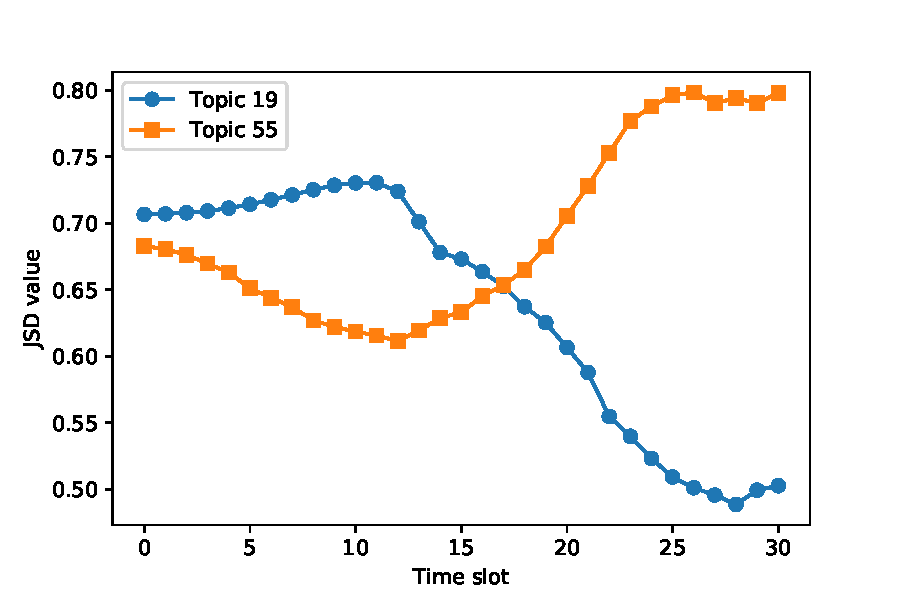
\includegraphics[scale=0.7]{JSgraph.pdf}
\tiny
\begin{tabular}{|p{7cm}|p{7cm}|}
\hline \bf LDA Topic 19 & \bf LDA Topic 55 \\ \hline

'rank', 'matrices', 'norm', 'tensor', 'entries', 'decomposition', 'columns', 'column', 'subspace', 'spectral', 'singular', 'completion', 'privacy', 'row', 'svd', 'trace', 'sparse', 'vectors', 'rows', 'private', 'product', 'diagonal', 'orthogonal', 'min', 'minimization', 'exact', 'factorization', 'differential', 'nuclear', 'symmetric', 'missing', 'entry', 'subspaces', 'recover', 'vec', 'tensors', 'arxiv', 'estimation', 'guarantees', 'noise', 'covariance', 'condition', 'power', 'projection', 'recovery', 'diag', 'norms', 'differentially', 'frobenius', 'k2f'
&
'noise', 'signal', 'components', 'component', 'filter', 'signals', 'source', 'filters', 'coefficients', 'mixture', 'noisy', 'sources', 'ica', 'separation', 'mixtures', 'filtering', 'variance', 'estimated', 'transform', 'blind', 'power', 'coding', 'wavelet', 'estimation', 'basis', 'snr', 'denoising', 'higher', 'invariant', 'gaussians', 'mixing', '1997', 'sensor', 'samples', 'unknown', 'orthogonal', 'fig', 'measurements', 'estimates', 'nonlinear', 'normalization', 'adaptive', 'overcomplete', 'equivalent', 'complex', 'correlated', 'elements', '2000', 'distributed', 'filtered'
\\ \hline

\end{tabular}
\caption{Models trained with the NeurIPS dataset with 60 topics for both DTM and LDA: Word distribution of DTM topic 0 at time slices T=0, 5, 10, 15, 20, 25, and 30 is shown in the first table. The last table shows the word distributions of LDA topics 19 and 55, respectively, and both curves in the graph are the JS similarity measure of DTM topic 0 with LDA topics 19 and 55. This is a graphical representation of two fragmented LDA topics related to one single DTM topic.}
\label{fig:fragmentation}
\end{center}
\end{figure*}

\section{Estimation of Connections from Fragmented LDA Topics}

To extract DTM topic information from LDA, we use the inverse approach, which is to try to extract relevant information from LDA and, if the extracted information matches DTM's topics, then we can say that this technique is a good way to extract DTM's topics using LDA. For this comparison, we used below mentioned approaches:

\begin{itemize}
\item Overall correlation of LDA topics
\item Time series topic correlation
\end{itemize}

Fragmentation means a single DTM topic contains two or more partial LDA topics. LDA topics that are related to a single DTM topic are similar in some aspect, so calculating the correlation among fragmented LDA topics is a good starting point. The correlation coefficient calculates the strength of the relationship between the relative movements of two variables, and the variables in this case are LDA topics that are calculated from the topics distribution $\theta_{dk}$. As DTM is time-dependent, it is better to also check the correlation of LDA topics in a series by categorizing documents with respect to time and then aggregating the correlation coefficient of each time slice.

\section{Topic Popularity Analysis}
Lastly, the time series topic popularity, which is the second important information offered by DTM, can be extracted from the LDA topics. After calculating document-topic distribution $\theta_{dk}$, the documents are categorized with the same time series information as used in DTM. Then, we calculate the estimated number of documents for each topic in a time series manner ($N^t_k$ using Equation \ref{eq:N_k_t}) and construct a graph that is comparable to the DTM topics popularity information.

%%%%%%%%%%%%%%%%%%%%%%%%%%%%%%%%%%%%%%%%%%%%%%%%%%%%%%%%%%%%

\chapter{Experiment}
The experimental process started with collecting and preparing the datasets. Then appropriate configurations for DTM and LDA models were selected. After training both models with one dataset set at a time, we extracted topic-word distributions and word probabilities. These word probabilities were used for computing the JS divergence from which we made the JS similarity-based graphs. We computed the overall correlation and time series correlation for one of the datasets in one of the configurations to try to extract the DTM time series topic distributions from the LDA topics. We also plotted population graphs from this configuration's inference part to compare it with the DTM topics.

\section{Datasets}
Three different datasets were used in this experimental procedure and these are categorized as large document dataset, normal document and short text dataset to check the behaviour of topic models with different type of datasets. 

\textbf{NeurIPS}: This dataset consists of research papers from the conference of neural information processing systems (NeurIPS formally known as NIPS) from 1987, when the conference first started, to 2017. There are 7242 documents in this dataset with three unrecognizable, so a total of 7239 research papers were part of the dataset used in training of DTM and LDA.  In the preprocessing, we removed stop words (e.g., the, a, an, in) using the \textit{nltk.corpus}\footnote{\url{http://www.nltk.org/api/nltk.corpus.html}} python package, special characters (e.g., \$, @, \%, \&), URLs, and words having only two characters because most two characters words do not have concrete meanings (e.g., up, vs, ha). A research paper is relatively a big document ranging from 4 to 10 pages, sometimes more so this dataset is categorized as large documents dataset. 

\textbf{News}: This dataset\footnote{\url{https://components.one/datasets/all-the-news-articles-dataset/}} consists of 204,135 news articles from 18 American publications and each row has columns "id", "title", "author", "date", "content", "year", "month", "publication", "category", "digital", "section", and "url". Each row represents one single news article. Some of the entries may have a \textit{NULL} value for an article. There are 191,530 articles that have date information and also the distribution of articles over the years is sparse. We therefore selected articles published in 2016 and 2017, totaling 95,997 and 75,034 respectively. Thus, a total of 171,031 news articles were divided into 24 time slices based on the month-year parameter for DTM training and the inference of LDA. The same preprocessing steps were applied to this dataset as mentioned above for the NeurIPS dataset. On average a news article is one page document so we categorized it as normal documents dataset.

\textbf{Twitter}: The last dataset is Tweets2011\footnote{\url{https://trec.nist.gov/data/tweets/}} dataset of more than three million English tweets sampled between January 23 to February 8, 2011. As the original dataset consists of the publicly available tweets in that period which means that tweets are in many languages. We used the Python library \textit{langdetect}\footnote{\url{https://pypi.org/project/langdetect/}} to extract the English tweets. There is character limit for a single tweet and tweets are very short piece of text so this dataset is categorized as short text dataset. Usually, a tweet is a messy piece of text, so some preprocessing is desirable as the first step in cleaning this data.
We therefore removed stop words, usernames, URLs, special characters, and two-letter words because mostly two characters words do not have concrete meaning (up, vs, ha, RT and more). We applied hashtag pooling for training process of models and day-hashtag pooling in inference part.

\section{Models Configuration}
We have some hyper parameters that need to be fixed before training of topic models. 

\textbf{LDA} implementing the stochastic variational Bayesian method of \cite{mimno2012sparse} in Java with three different numbers of topics $K$, 1000 docs per batch (also known as mini-batch size), and 1000 iterations was trained with the above-mentioned datasets one at a time.

\textbf{DTM} was implemented using the gensim.model.wrappers with DTM implementation \footnote{\url{https://github.com/magsilva/dtm}} in C and C++. We trained the DTM on three different numbers of topic configurations with each dataset.

\textbf{Topics:} We selected three values (30, 60, and 90) for the hyperparameter ``number of topics'', denoted as $K$. We trained the DTM and LDA with one dataset at a time and with one of the $K$ values.

The experiment environment was Ubuntu 16.04 for the operating system, two Intel 80n E5-2630 (2.40 GHz) with eight cores for the central processing unit, and Python and Java for the LDA implementation and Python and C/C++ for the DTM implementation.

%%%%%%%%%%%%%%%%%%%%%%%%%%%%%%%%%%%%%%%%%%%%%%%%%%%%%%%%%%

\chapter{Results}
This section is divided into multiple sub-sections; each part explains the different aspect of our research.

\section{Training Time Cost}
As mentioned earlier, the computational cost for DTM is higher than LDA;  however, to determine the difference in training time, we conducted a small sub-experiment in which we trained both the DTM and LDA models with multiple-size documents and hyperparameter value $K$, which is the number of topics. The dataset used for this experiment was the ``Twitter'' dataset. Preprocessing cleaning and hashtag pooling were applied before training.

\begin{figure}[h!]
\begin{center}
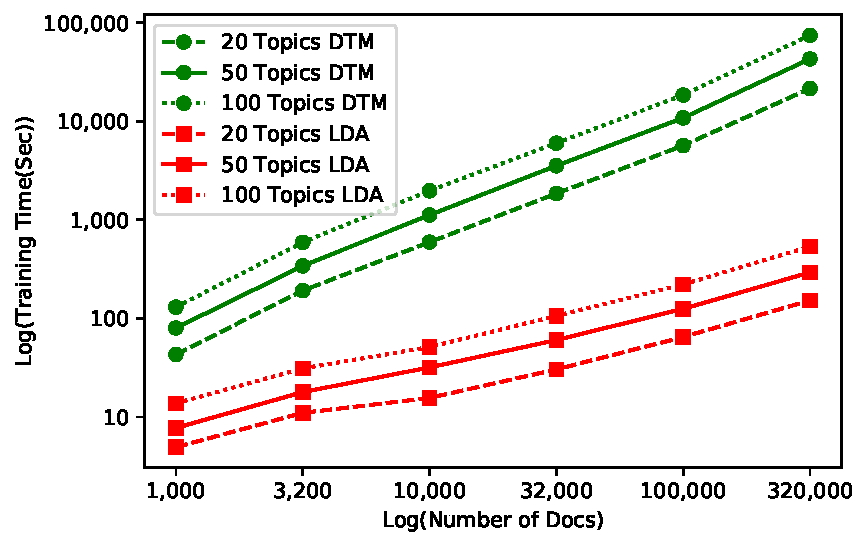
\includegraphics[scale=0.8]{costGraph.pdf}
\caption{This graph is in logarithmic scale to fit higher values into the figure. The x-labels are the number of documents on which the models were trained and y-axis is the time in seconds that each model took for training.}
\label{fig:trainingTime}
\end{center}
\end{figure}

Figure \ref{fig:trainingTime} shows that increasing the number of documents or the number of topics increase the training time. We see a roughly linear increase in time for both models. For small datasets, the training time of DTM was 10 times more than LDA and exceeds \textbf{``100 times''} for big datasets. Normally in NLP topic modeling problems, datasets are relatively bigger in size. We can therefore say that DTM will take around 100X more time for training compared with LDA under the same conditions.

\section{Topic Drifting}
Topic drifting is fundamental information extracted from DTM. A single DTM topic consists of topics at each time slot. For clarity, let us call such a time-slice-topic the ``focus'' of the DTM topic. The focus of a DTM topic changes over time, as shown in the first part of Figure \ref{fig:fragmentation}, where the focus changed from ``Signal Processing'' to ``Tensor Decomposition'' by the end. This is called topic drifting or topic transition. We calculated the total unique vocabularies for each DTM topic. $V_s$ is the vocabulary size, which is the number of unique words that appeared in all time slots topic-word distributions of a single DTM topic. The minimum vocabulary size for any topic was 50. If any topic had $V_s$ close to this number, it means there were few new words in the different time slot topics. In short, the focus of this specific topic remained the same and there was no topic drifting.

\begin{table}[h!]
\begin{center}
\begin{tabular}{|c|c|c|c|c|}
\hline \textbf{Dataset} & \textbf{Topics} & $K(V_s > 70)$& $K(V_s > 90)$ & $K(V_s > 120)$ \\ \hline

\multirow{3}{*}{NeurIPS}  & 30 & 13 & 8 & 0 \\ & 60 & 58 & 56 & 11  \\ & 90 & 90 & 90 & 90  \\ \hline
\multirow{3}{*}{Twitter}  & 30 & 3 & 1 & 0 \\ & 60 & 3 & 0 & 0 \\ & 90 & 1 & 0 & 0 \\ \hline
\multirow{3}{*}{News}  & 30 & 29 & 20 & 5 \\ & 60 & 57 & 33 & 1 \\ & 90 & 83 & 37 & 2 \\ \hline

\end{tabular}
\caption{$V_s$ is the vocabulary size, which is the number of unique words that appeared in all time slot topic-word distributions of a single DTM topic. Minimum $V_s$ is 50.  $K(V_s > 70)$ means the number of DTM topics having a vocabulary size of more than 70. Similarly $K(V_s > 90)$ and $K(V_s > 120)$ mean the number of topics having a vocabulary size of more than 90 and 120, respectively. }
\label{table:topicDrifting}
\end{center}
\end{table}

In Table \ref{table:topicDrifting}, $K(V_s)$ values for the Twitter dataset are very low, which means there were not many new words in the DTM topics and the focus of the topics remained the same over all times. This implies that DTM topic drifting for the Twitter dataset is negligible. And $K(V_s)$ values for the DTM trained on NeurIPS and News dataset were relatively high, which implies that there were topic drifting phenomenons.

\section{JS Analysis}
To extract the information overlap of the DTM and LDA topics, we computed JS values using Equation (\ref{eq:jsd}) for all the datasets in all topic configurations. The JS value is bounded by 0 and 1 for two distributions, where 0 means both distributions are identical and 1 means there is no similarity between both probability distributions. A threshold value of 0.7 was selected and any DTM topic distribution having a JS value lower than or equal to this threshold when measured with the LDA topic distributions was part of the related topic ``RT'', fragmented topic ``FT'', and others. A summary of this analysis is set forth in Table \ref{table:JStable}.

\begin{table}[h!]
\begin{center}
\begin{tabular}{|c|c|c|c|c|c|c|}
\hline \textbf{Dataset} & \textbf{Topics} & \textbf{RT}& \textbf{FT} & \textbf{F 2} & \textbf{F 3} & \textbf{F 4 \& more} \\ \hline

\multirow{3}{*}{NeurIPS}  & 30 & 17 & 4 & 3 & 1 & 0 \\ & 60 & 42 & 16 & 11 & 5 & 0  \\ & 90 & 69 & 28 & 25 & 2 & 1 \\ \hline
\multirow{3}{*}{Twitter}  & 30 & 5 & 0 & 0 & 0 & 0 \\ & 60 & 11 & 1 & 1 & 0 & 0 \\ & 90 & 14 & 3 & 2 & 1 & 0 \\ \hline
\multirow{3}{*}{News}  & 30 & 8 & 1 & 1 & 0 & 0 \\ & 60 & 24 & 2 & 2 & 0 & 0 \\ & 90 & 42 & 4 & 4 & 0 & 0 \\ \hline

\end{tabular}
\caption{DTM and LDA trained on ``Dataset'' with ``Topics'' configuration one at a time, ``RT'' is the total number of DTM topics having a relationship with the LDA topic/s. ``FT'', ``F 2'', ``F 3'', and ``F 4 \& more'' are the number of DTM topics having a JS relationship with two or more LDA topics, only two LDA topics, only three LDA topics, and more than three LDA topics, respectively.}
\label{table:JStable}
\end{center}
\end{table}

Table \ref{table:JStable} shows that a negligible amount of ``FT'' fragmented topics was found for the datasets ``News'' and ``Twitter'' because most news articles and tweets are instantaneous responses of some events, and these topics die within short period of time; in other words, we see other tweets and article about other events. Due to this focus shifting behavior of the documents, DTM cannot accurately locate topic transitions over time. That is why very few fragmented topics were found for these datasets. Related topics ``RT'' are comparatively higher for ``News'' as compared to ``Twitter'' dataset because the domain of tweets is huge; it could be anything ranging from personal (My pet is very cute) to political (US president announced a restriction on trade agreement with China), whereas the News articles domain is restricted compared with Twitter. We can therefore have many topics in the Twitter dataset. Due to random initial conditions of both DTM and LDA, it is safe to say that both models could come up with different topics. As mentioned, the News dataset domain is restricted so we see high topic overlapping values in this dataset's results.

The domain of the ``NeurIPS'' documents focus on a few subjects (machine learning, artificial intelligence, computational neuroscience, etc.), so related topics ``RT'' values are very high compared with other dataset configurations. High fragmented topic ``FT'' values can be seen for the ``NeurIPS'' dataset in Table \ref{table:JStable} because research papers tend to follow previous researches or somehow align with previous research papers. That is why we can see a well-defined topic transitions in the DTM topics, as shown in Fig \ref{fig:fragmentation}.

In all the datasets, increasing the number of topics resulted in an increase in ``RT'' and ``FT'' values.

\begin{table}[ht!]
\begin{center}
\begin{tabular}{|c|c|c|c|c|c|c|c|}
\hline \textbf{Dataset} & \textbf{DTM} & \textbf{LDA} & \textbf{RT}& \textbf{FT} & \textbf{F 2} & \textbf{F 3} & \textbf{F 4 \& more} \\ \hline
NeurIPS & 30 & 1000 & 25 & 20 & 3 & 7 & 10 \\ \hline
\end{tabular}
\caption{A special configuration with DTM topics and LDA topics was also examined to analyze the behavior of a LDA model trained with a high number of topics.}
\label{table:JS30DTM1000LDA}
\end{center}
\end{table}

If we increase the number of topics in LDA, we get more and more fragmented topics, which means that topics are further divided into smaller and more focused themes. DTM's computation cost restricts us from increasing the number of topics, so we cannot get the type of topics that we can get from LDA with a very high $K$ hyperparameter.

\section{Overall Correlation}
Due to fragmentation detection, being part of a single DTM topic, fragmented LDA topics should have some relationship with each other. For example, the documents that have a high probability of topic 0 shown in Figure \ref{fig:fragmentation} in the DTM analysis should have a high probability for topic 19 and 55 in the LDA analysis as compared to other topics. This phenomenon leads to the hypothesis that \textit{"fragmented topics have similar distributions"}. Therefore we find the overall correlation coefficient for all the fragmented topics extracted from the LDA model trained on the ``NeurIPS'' dataset with $K = 60$.
After training the model, topic distribution for each document was calculated using the method described in Chapter 3. This topic distribution gives us insights into the relevance of each document with each topic. Document-topic probabilities of the fragmented topics were used as variables to calculate the overall correlation.

The analysis showed no significant results and most of the correlation values were around 0, which means there is no linear relationship between fragmented topics, with few exceptions ranging up till ``0.44'' indicating some relation but not significant enough to prove our hypothesis.

\section{Time Series Correlation}
We also checked the correlation in a time series manner because fragmented topics have time series effects. For example Figure \ref{fig:fragmentation} shows that the JS similarity for both topics was close until the 15th time slot and the DTM topic was biased towards topic 19 as compared to topic 55 around at the end. Therefore it was also, worth checking the relationship of fragmented topics in a time series manner to further explore our hypothesis.

We split the document-topic distribution according to the time slots, checked the correlation of the fragmented topics in each time slot, and then made a graph to view the correspondence of the time series correlation graph with JS graphs. The resultant graphs showed no strong relationship between fragmented topics and we could not find evidence to prove our hypothesis \textit{fragmented topics have similar distributions}.

\section{Time Series Topic Popularity}
Topic popularity is the fundamental information that can be extracted from a topic model and, especially in the case of DTM, time series topic popularity is estimating the number of documents for each topic at each time slice. We can easily construct this information into a self-explanatory graphical representation of topic popularity. For this analysis, we selected the 60 topics of the ``NeurIPS'' configuration. Then $\gamma$ distributions for the documents were calculated which gives the probability of each topic for each document. Time-depended summation over the topics then gives us the estimated number of documents for each topic at each time slot. 

We can also extract this information from LDA with a few extra steps. First, we trained the LDA with the same dataset and got topics with the same 60-topic configuration. Before getting the $\theta_{dk}$ distributions for the documents, we saved the date information with the documents so that when we get the $\theta_{dk}$ distributions, we know the corresponding date of each document. With these distributions and dates, we applied time-dependent summation over the topics and got an estimated number of documents for each topic at each time slot. Afterward, we plotted this information into graphs. To reduce noise effects and to make the graphs smooth, we used the Savitzky-Golay digital filter \cite{william1990sgfilter}.

\begin{figure}[h!]
\begin{center}
\begin{tabular}{cc}
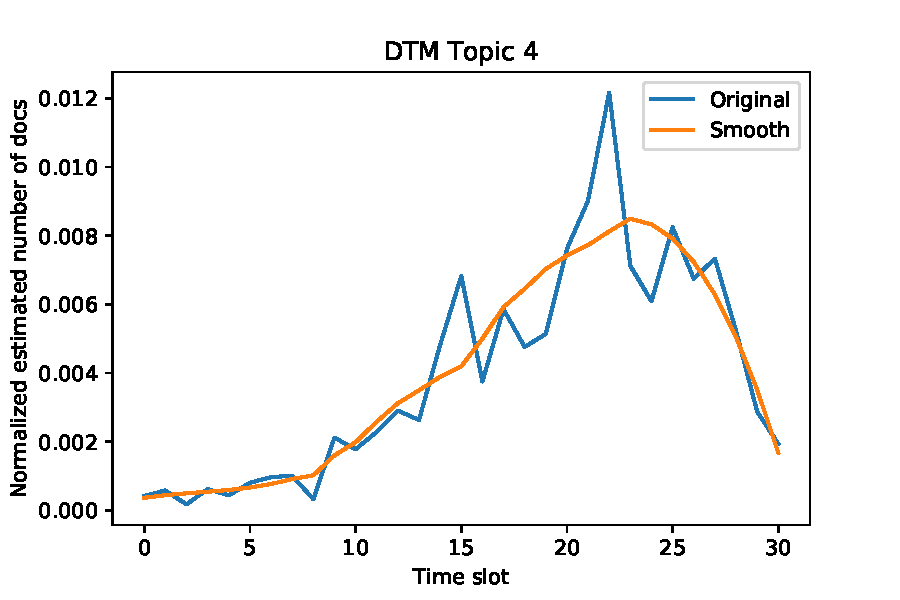
\includegraphics[scale=.5]{DTMpopulationTopic4.pdf} &
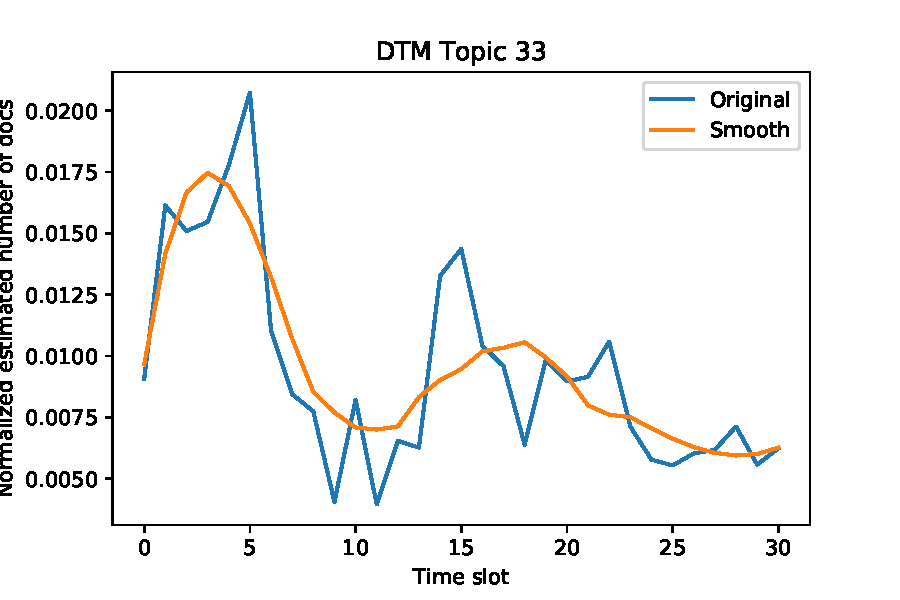
\includegraphics[scale=.5]{DTMpopulationTopic33.pdf} \\
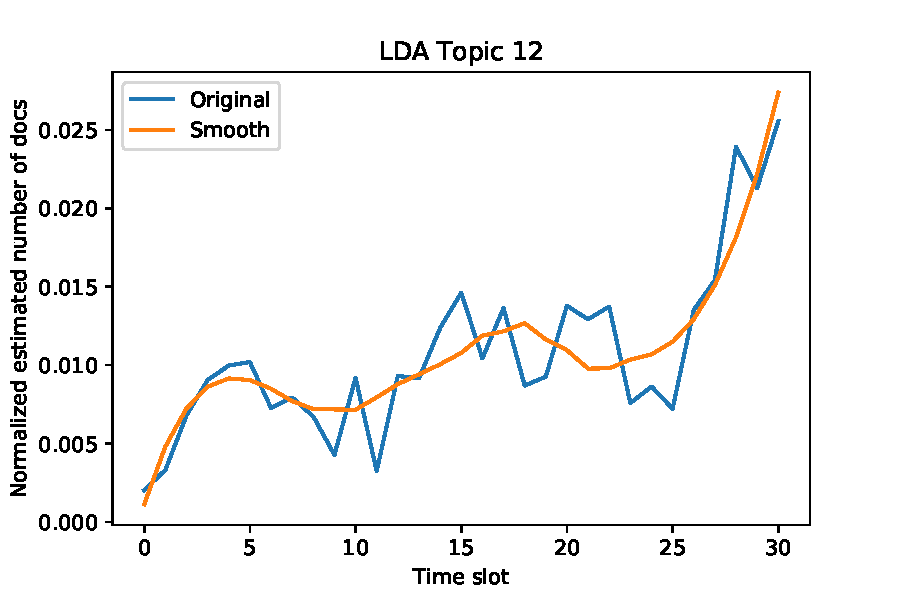
\includegraphics[scale=.5]{LDApopulationTopic12.pdf} &
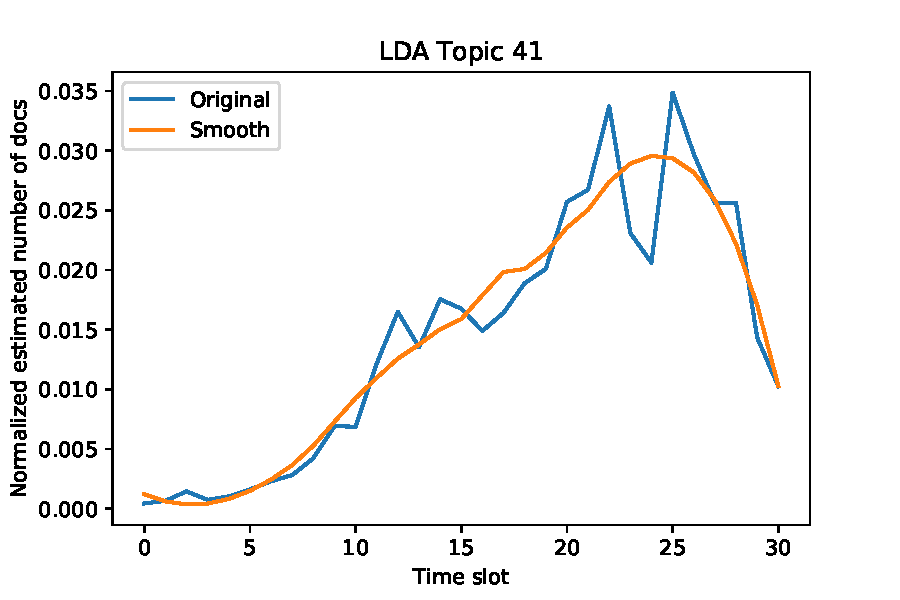
\includegraphics[scale=.5]{LDApopulationTopic41.pdf}
\end{tabular}
\caption{Number of documents for each time slot estimated from $\gamma$ and $\theta$ distributions of the documents for DTM and LDA respectively. Two topics from each model are shown here. The horizontal axis shows the time slot number and the vertical axis is the normalized estimated number of documents for these topics.}
\label{fig:populationGraphs}
\end{center}
\end{figure}


Figure \ref{fig:populationGraphs} shows the time series topic popularity of both the DTM and LDA topics. The top two graphs in the figure are of DTM topics 4 and 33, respectively, and the bottom graphs show the time series popularity of LDA topics 12 and 41. These graphs show that the time series topic popularity can be extracted from DTM as well as LDA.

%%%%%%%%%%%%%%%%%%%%%%%%%%%%%%%%%%%%%%%%%%%%%%%%%%%%%%%%%%

\chapter{Discussion}
 Topic drifting and time series topic popularity are the main aspects of this research and we compared these aspects for DTM and LDA. In this section, we discuss a few important points of both concepts as they apply to DTM and LDA.

\section{Topic Drifting}
There is no topic drifting for DTM trained on the ``Twitter'' dataset ({Table \ref{table:topicDrifting}}), so the only important information which can be extracted from such datasets is the time series topic popularity which can be extracted using LDA, thus we should avoid the high cost of using DTM as the topic model.  

For the ``NeurIPS'' dataset, the topic drifting increased as we increased the number of topics for the DTM model. All 90 topics have  $V_s$ greater than 120 words for this dataset in the 90-topic configuration (Table \ref{table:topicDrifting}), which means there was high topic drifting and this high topic drifting information provides rich insights into topic transitions. Therefore, if we specifically want to examine topic drifting over time in such datasets, DTM is a promising model to use; however, we must keep in mind that if our goal is topic popularity, then LDA is a far better option. 

From the same table, we also experienced the drifting in the topics extracted from the ``News'' dataset, but the vocabulary size is comparatively low for the higher number of topics. This means that there exists topic drifting with such datasets, but it may not be as effective as we desire. More subjective analysis based on research problem can help determine if DTM is a good option or not. One interesting insight should be mentioned here; DTM tends to forcefully find the topic transitions in some cases. For example, in the 30-topic configuration for the News dataset, topic 29 started with words like \textit{(archive, team, collection, sign, projects, machine, contains, lost, providing, comment, websites, collections, wayback)}, but the word distribution at the end was \textit{(travel, airport, flight, air, trip, passengers, flights, travelers, plane, airlines, united, airline, passenger)}. Looking at these distributions, we can say that DTM failed to extract the correct topic drifting over time for topic 29.

\section{Topic Popularity} 
We have $\gamma$ and $\theta$ distributions for DTM and LDA, respectively. Once the models are trained, we can extract these distributions for any document and these distributions provide the topics proportion for each document. We can then estimate the number of documents for each topic using the method described in Chapter 3 for the LDA model and, with this time series document estimation, we can construct a time series topic popularity graph. Similarly, we can construct this graph for DTM topics. Thus, this fundamental information can be extracted using both models. 

Notably, the topic popularity extracted from DTM is a little vague because DTM topics have topic transition information embedded with the topics. For example, topic 4 shown in Figure \ref{fig:populationGraphs} has word distribution \textit{(retrieval, content, query, queries, text, relevance, documents, semantic, words, document, lda, relevant, collection, word, latent, topics)} at $T= 0$, which is about ``Information retrieval from documents'' and the word distribution at $T= 30$ is \textit{(topic, topics, document, lda, word, documents, words, latent, dirichlet, text, models, allocation, model, corpus, gibbs, modeling, blei)}, which is about ``Document analysis with LDA''. Similarly, DTM topic 33 was about ``Language structure rules'' in initial time slots and the theme of the topic was changed to ``Question-answer reasoning'' around the end. But, if we are looking for the popularity graph of a topic ``Information Retrieval'', then LDA topic 12 is an accurate option. Similarly, LDA topic 41 is more accurate if we want to see the popularity graph of the topic ``Variational topic model LDA'' because there is no topic drifting in LDA. The word distribution for LDA topic 12 is \textit{(word, words, language, sequence, recurrent, text, lstm, rnn, semantic, context, attention, table, vectors, embedding, sequences)} and for LDA 41 is \textit{(latent, inference, topic, sampling, mixture, variational, posterior, gibbs, dirichlet, topics, lda, markov, document, likelihood, prior, distributions)}. Because of the topic transition information embedded with DTM topics, it is not the best option for time series topic popularity information.

%%%%%%%%%%%%%%%%%%%%%%%%%%%%%%%%%%%%%%%%%%%%%%%%%%%%%%%%%%%

\chapter{Use Case in Social Media Analysis}
%News extraction from Twitter data is a hot topic. But can we extract much more than just news? 
Since the user-generated content platforms such as Twitter are becoming a more common news source \cite{bruns2012researching}, news extraction from such documents has attracted attention as an import task \cite{hu2012breaking, brems2017personal}.
Meanwhile, many kinds of other topics are talked on Twitter than popular news \cite{zubiaga2015real, lee2011twitter}. 
In this chapter, we conduct an experiment to find, either news is the only information which can be extracted from Twitter data or it contains much more insights about real life events. So, we used proposed  method (LDA topic popularity) for analysis of Twitter’s raw content. After pre-processing of tweets data, we apply hashtag pooling and extract topics using LDA without modifying its core machinery. In the second part, estimated number of tweets per day and correlated top hashtags for each topic are calculated using day-hashtag pooling. Finally, time series topic popularity graphs are constructed for topic analysis. Interesting results of bursty news detection, topic popularity, people’s way to perceiving an event, and before \& after affects of a specific event were found.

\section{Topics in Twitter}
Twitter has millions of users who try to sum up an event, trend or their emotions into few character's short post. Diverse users of twitter freely express their thoughts which leads to many topics. Extracting trends from tweet’s data could be very handy to know and understand better about real-life events because of huge dataset available and people’s interest in it. The application area of twitter is vast including many useful domains such as real-time events detection \cite{sakaki2010earthquake}, sentiment predication analysis \cite{tumasjan2010predicting}, understanding public health opinions \cite{karami2018characterizing}, time series topic popularity variation \cite{fukuyama2018extracting} and it's comparison with traditional media \cite{zhao2011comparing}. Over 85\% of topics are headline news or persistent news in nature when tweets data is classified for trending topics  \cite{kwak2010twitter}. These topics aren't just only news but also contain reasons and effects of specific events. Also, people's interest is directly proportional to intensity of a specific event and its effects on people's life. As we know millions of tweets are tweeted everyday so it is impossible to extract topics manually. Twitter has hashtag information to follow the trending topics and frequency of tweets per hashtag can give us some information about popularity of a hashtag. But, hashtag is a user generated string and can lead to many topics or sometimes irrelevant information related to one specific topic. So, we used time series topic popularity concept to find most of the useful information from twitter's raw data.

\section{Making Popularity Graphs}
The goal of this experiment is to extract topic trends in tweets data efficiently and analyzed visually. The first step towards our goal is to clean the tweets as much as possible in pre-processing, then we use hashtag pooling to make our documents relatively bigger in size as compared to single tweets. Next step is to apply LDA on hashtag pooled tweets data and extract the topics distribution and top words for each topic which convey the meaning of that specific topic. Before the inference, we apply day-hashtag pooling so that we could be able to track the topic trend on time series graph. Inference in this case, is estimating the total number of tweets belong to each topic in each document. As day-hashtag pooling is applied so estimated number of tweets $N^t_k$ can be calculated using Equation (3.1). The final step is to make graphs of estimated tweets along y-axis and time series along x-axis. In this method we also extract the top words of topics and top hashtags contributing in each topic for each document.

\section{Experiment Procedure}
To meet the expectation of this experiment which is trends analysis from twitter data. We used ``Twitter" dataset. Same preprocessing steps mentioned in Section 5.1 were performed here as well. Next step applied was hashtag pooling and after applying it we got 275,836 hashtag pooled documents. Then LDA with 1000 number of topics was trained on hashtag pooled documents. The training of LDA took one hour 17 minutes and 54 seconds and for the inference part the time for calculating $\theta_{dk}$ of documents for topics was just 16 minutes and 20 seconds.

\section{Twitter Topics Analysis}
Three parts need to be explained in this section. Different techniques were merged and implemented in this experiment so it is a good idea to discuss the findings step-vise and ultimately combine all the results to show it in presentable and easy form.

The parts are divided into three subsections and discussed in details bellow. First, topics generated by training of topic model LDA are discussed. Secondly, unique concept top hashtags for correlated topics is explained. In the last part of this section, Time series graphs along with top hashtags analysis is explained in details.

\subsection{Topics}
As already mentioned in previous section, 1000 topics as an input is used for hyper parameter $K$ and top 10 words are extracted from topic-word distribution because top 10 words of most of the topics are self explanatory and by just looking at those words we can come-up with topic category that topic belongs to.

\begin{table}[!ht]
\begin{tabular}{|p{0.5cm}|p{2.5cm}|p{10.5cm}|}
\hline  & \bf Topic & \bf Top words \\ \hline
1 & Music & song, listening, club, track, right, radio, home, hot, high, ill  \\ \hline
2 & Education & learning, education, past, language, driven, brush, lessons, intelligent, digg, arts \\ \hline
3 & USA & american, gov, spread, brotherhood, reform, barackobama, decades, democracy, 500, damon \\ \hline
4 & Climate & moon, fine, weather, baro, rising, speed, officialkimora, waning, sunrises, mostly \\ \hline
5 & Gadgets & gps, laptop, battery, watch, charger, nike, wifi, tablet, color, high \\ \hline
6 & Football & deal, suarez, club, carroll, kenny, player, transfer, players, request, luis \\ \hline
7 & Justin Bieber & newmusiclive, justin, bieber, made, tuesday, say, pattie, beiber, till, belieber \\ \hline
8 & Photography & photos, m4w, gallery, photographer, camera, w4m, stunning, fleur, photographic, kitty\\ \hline
9 & Gaming & xbox, trailer, ops, 360, famous, beta, protests, capcom, unlocked, brief \\ \hline
10 & Violence & kills, dead, weekly, iron, headshots, transforming, architects, slayer, tix, attack \\ \hline
\end{tabular}
\caption{Top words of topics}
\label{table:topic-word}
\end{table}

In Table \ref{table:topic-word}, very few of the total topics and top words of these topics are shown and summarization of these words into a title of the topic. For example, topic 1, from words like song, listening, track, and radio, it is obvious that this topic is related to music. Words of topic 2 are learning, education, language, lessons, and intelligent that clearly means that this topic refers to education in general and word distribution (american, gov, barackobama, democracy) is somehow related to USA for topic 3. So I can claim that we can easily come up with topic title from the top words of LDA generated topics which can be proved from other examples too. 

\subsection{Top Hashtags}

\begin{table}[!ht]
\begin{tabular}{|p{0.5cm}|p{2.5cm}|p{10.5cm}|}
\hline  & \bf Topic & \bf Top hashtags \\ \hline
1 & Music & nowplaying-2/3, nowplaying-2/8, np-1/27, nowplaying-1/27, nowplaying-2/2   \\ \hline
2 & Education & 8days-2/3, bring5friends-1/23, happybirthdayharry-2/1, twitition-1/27, welovestyles-1/23 \\ \hline
3 & USA & egypt's-2/5, egypt-1/28, scariestwordsever-2/5, jan25-1/29, sfo-2/6 \\ \hline
4 & Climate & news-1/32, nowwatching-2/4, aquarius-2/2, zodiacfacts-2/1, unknownwhat-1/26 \\ \hline
5 & Gadgets & twalue-1/25, lfc-1/30, americanidol-1/27, teamfollowback-2/8, worstpickuplines-2/2 \\ \hline
6 & Football & gwo-1/29, mbteamcl-2/2, global-2/7, nufc-1/31, aquarius-1/26 \\ \hline
7 & Justin Bieber & nmlbelieber-1/28, hosting-2/4, hosting-1/29, muchmusic-1/31, hosting-2/5 \\ \hline
8 & Photography & news-1/23, thegame-2/2, np-2/2, fail-2/7, neversaynever3d-1/24\\ \hline
9 & Gaming & twibbon-1/24, twibbon-2/7, magistream-2/5, blackandyellow-2/7, thegame-2/2 \\ \hline
10 & Violence & jan25-2/2, egypt-2/3, jan25-2/1, jan25-2/4, jan25-2/3 \\ \hline
\end{tabular}
\caption{Top hashtags of topics}
\label{table:topic-hashtags}
\end{table}

LDA generated topics seems self-explanatory but is this information enough to claim that twitter users truly talked about these topics? Some supporting evidence can extracted to prove that people were really interested in these topics and actually tweeted about these topics. For this, some tweaks in inference were applied to extract that supporting evidence. In the inference part, a new dataset was created from our original twitter dataset by using day-hashtag pooling technique. In this dataset, all the hashtags having more than 10 tweets were included to make a relatively large and efficient document dataset for topics correlation with hashtags. All the tweets with one hashtag of a single day were merged into one document and in total there were 9686 documents. LDA model which was trained on original dataset was applied to this dataset for hashtag relation with topics. $\theta_{dk}$ of each topic for every document was calculated. Then using equation 3.1, estimated number of tweets for each topic were calculated. Once estimated number of tweets are calculated, conclusions about the document (in this case made with respect to hashtags) relevance with topics can be easily made that indicates hashtag relevance with topics.

In Table \ref{table:topic-hashtags}, same topics were chosen as in previous table (Table \ref{table:topic-word}) for this analysis. Top hashtags are shown as ``hashtag-month/date''. Some topics have strong correlation with their corresponding top hashtags, which states that people were interested and actually talked about these topics e.g top hashtags for topic ``Music'' are nowplaying, np. Another interesting example here is about topic ``Violence'' that has jan25, egypt as top hashtags which indicates riots happened in Egypt and known as January25 movement. But some random hashtags as top hashtags can also be seen for some of the topics, means Twitter users maybe used the words related to these topics in general but didn't explicitly had interest in these topics e.g. (8days, bring5friends, happybirthdayharry for topic ``Education''). 

\subsection{Time Series Graphs}
Tweet count estimation is an essential and valuable piece of information for better understanding. There were 425906 tweets in total of 9686 documents between time duration of 17 days (Jan 23 - Feb 8) in inference dataset. So around 25 tweets per topic each day is the equally average value. A very basic generalization is used here just to see the popularity of a topic that is, if the number of estimated tweets is higher than the average value then it implies people were more interested in this topic and topic was popular. \\

\begin{figure}[!ht]
\begin{center}
    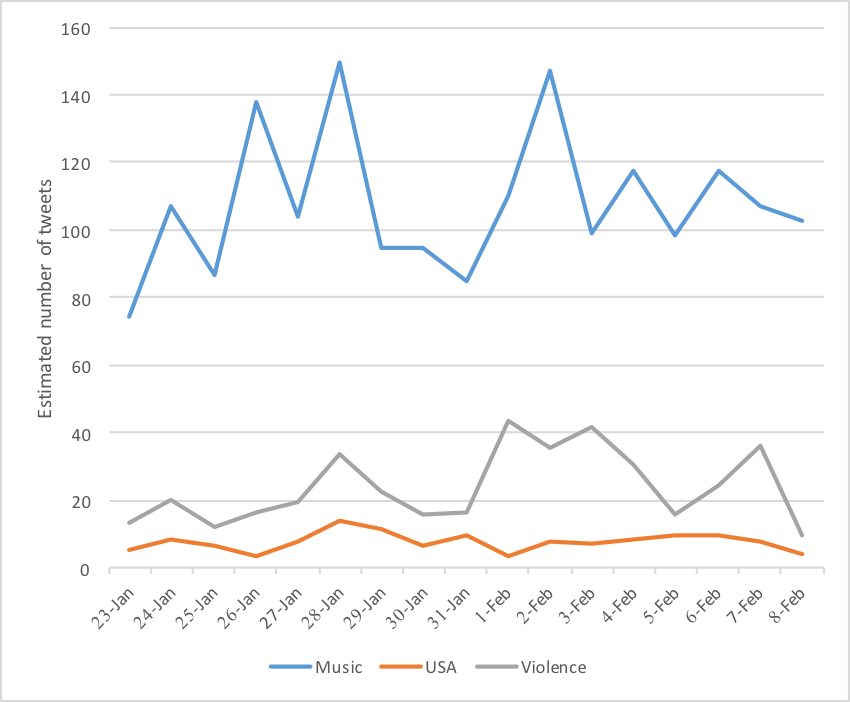
\includegraphics[scale=0.75]{graph1}
\caption{Inference dataset created by keeping time information into account. Tweet count estimation $N_k^t$ was calculated using Equation (\ref{eq:N_k_t}) by applying trained LDA on inference dataset. X-labels are dates and y-axis is estimated number of tweets. Only topic 1, 3, 10 from Table \ref{table:topic-word} \& \ref{table:topic-hashtags} are shown here.}
\label{fig:hashtag-related}
\end{center}
\end{figure}

\begin{figure}[!ht]
\begin{center}
    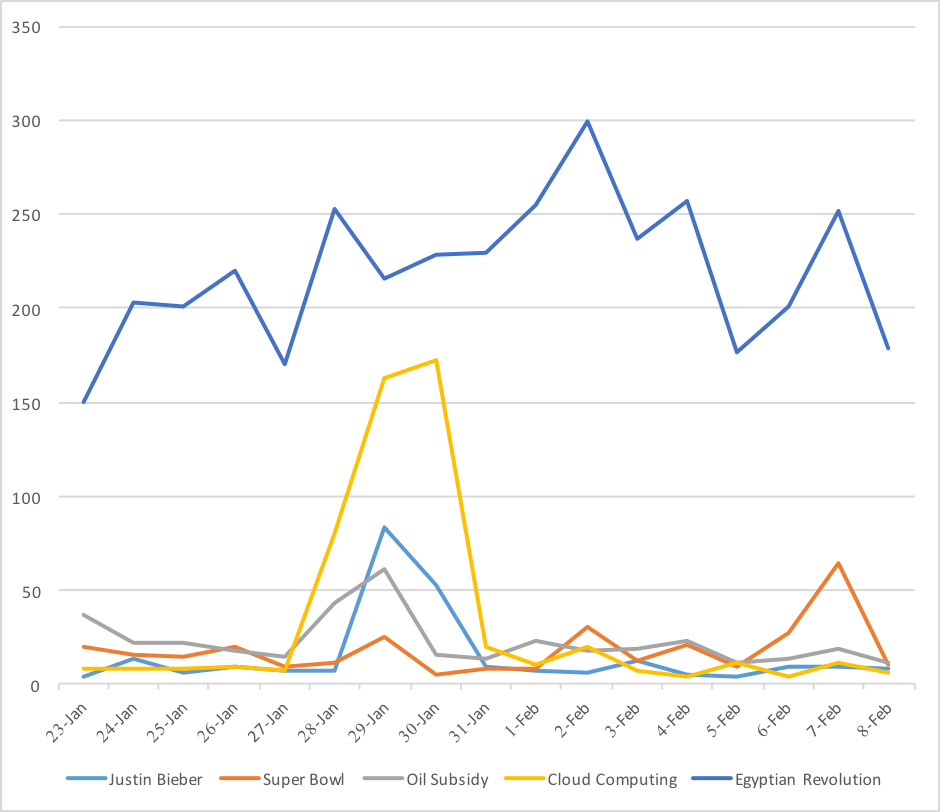
\includegraphics[scale=0.7]{graph2}
\caption{Topic popularity, burty topic detection, duration and peak of burstiness can be observed visually.}
\label{fig:tweet-topic-count}
\end{center}
\end{figure}


\begin{table*}[ht!]
\begin{tabular}{|p{0.5cm}|p{3.2cm}|p{3.2cm}|p{3.2cm}|p{3.2cm}|}
\hline  & \bf Top Words & \bf Top hashtags & \bf Sample Relevant Tweet &\bf Topic Statement \\ \hline

1 & wacky, guitar, soca, ensemble, orgy &  nmlbelieber-1/29, nmlbelieber-1/30, muchmusic-1/29, nml-1/29, nml-1/30 & Justin Bieber on NewMusicLive this Tuesday has made me a NMLBELIEBER & Justin Bieber performed on New Music Live \\ \hline

2 & ugh, alcoholic, failure, cans, woke & superbowl-2/6, superbowl-2/7, steelers-2/7, steelers-2/6, sb45-2/7  & There are many Super Bowl Parties this Sunday around the Plymouth area at the bars and restaurants. & Super bowl parties    \\ \hline

3 & oil, obama, cnn, funding, response & cars-2/3, cars, 2/7, us-2/1, whatif-1/27, us-1/29 &  NYTimes: Obama’s Bid to End Oil Subsidies Revives Debate & Oil price subsidy statement by obama \\ \hline

4 & computing, couldcomputingexpo, billion, infrastructure, inc & cloud-1/28, news-2/3, cloud-1/29, cloud-2/2, services-2/2 &   Data Center Links: PEER 1, Telx, IBM, Unisys: IBM Launches \$42 Million Cloud Computing Cente... & Cloud Computing service launch by IBM \\ \hline

5 & news, video, facebook, live, blog & egypt-1/31, jan25-2/2, jan25-2/1, egypt-1/29, egypt-2/1 & "Internet is a gift from God for all of ""Egyptians"". They shut it down and We were just ""Gyptians" & Social Media played an important role in egyptian revolution  \\ \hline
\end{tabular}
\caption{Topic statement from top words, top hashtags and relevant tweet of topics}
\label{table:top-hashtags-word-count}
\end{table*}

From Table \ref{table:topic-word} and \ref{table:topic-hashtags}: topic 1, 3 and 10 have strong correlation of top words and top hashtags. But calculating estimated number of tweet per day and visualizing it shows the actual popularity of the topics. In Figure \ref{fig:hashtag-related}, ``Music'' which is topic 1 in Table \ref{table:topic-word} \& \ref{table:topic-hashtags} was way much popular topic as compared to others whereas topic USA which is topic 3 in both Tables is bellow average which means people were not much interested in USA's statements about Egypt on jan25.

The most interesting part of this experiment is \textbf{Time  Series Topic Analysis}. From Figure \ref{fig:tweet-topic-count}, that has date at x-axis and estimated number of tweets on y-axis, topic transition of actual events over time and people's interest in these events can been analyzed. Bursty topics and how high the burst value is can also be found by this graph analysis. 

For example, in Figure \ref{fig:tweet-topic-count}, topic ``cloud computing'' which is topic number 4 in Table \ref{table:top-hashtags-word-count} has a very high burst on January 29-30 and relevant tweet confirmed the reason of this burst which was a real life event. Similar bursty trends with topic justin bieber, super bowl and oil subsidy which are topic 1, 2 and 3 respectively in Table 3 can be observed by looking at the graph \ref{fig:tweet-topic-count}. 

An interesting thing observed in this experiment is, actual reasoning and some insights of an event can be discovered that may not be found by news articles or other source of information in real life e.g. social media played a very important role in the Egyptian revolution 2011 which can be seen in Figure \ref{fig:tweet-topic-count} as "Egyptian Revolution" and topic 5 in Table \ref{table:top-hashtags-word-count}. 

\section{Findings}
In this experiment, a technique was developed to extract topic trend transition in graphical representation from Twitter data without modifying the original machinery of LDA along with the help of hashtag pooling. Calculating estimated number of tweets for each topic tells us the actual popularity of the topics. This experiment also shows that with this technique we can detect not only bursty topics but also the level and interval of burstiness. Top hashtags correlation with topics reflects the focus of topics. Analyzing top words of topics, top correlated hashtags and estimated number of tweets all together, not just events duration but also the reasons and after effects of an event or at least what and how people's reaction was about a specific event happened in real-life can be found. I counter checked these results with the original tweets and information available on other platforms e.g. news articles, blog posts etc for authenticity. 

In contrast to Koike's et al. \cite{koike2013time} work where high cost DTM was used, we applied LDA and extracted similar information which means similar kind of results can be achieved by using LDA as compared to DTM when it comes to topic popularity analysis.

%%%%%%%%%%%%%%%%%%%%%%%%%%%%%%%%%%%%%%%%%%%%%%%%%%%%%%%%%%%

\chapter{Conclusion}
In this research, we executed a comprehensive study on the time series analysis of the popular topic models DTM and LDA. Our research focused on the fundamental time series information of topic drifting and topic popularity. To compare DTM and LDA, we tried to extract this information from the topic distributions of both models. Multiple datasets along with multiple topic configurations were used in this research.

We performed social media analysis experiment (Chapter 8) by using LDA and compared it with previous work in which similar type of problem was analyzed by using DTM. We were able to extract time series topic popularity, bursty topic detection, level and interval of burstiness. With this experiment, we can conclude that similar kind of results can be achieved by using LDA as compared to high cost DTM when it comes to topic popularity analysis.

Our findings are:

\begin{itemize}
\item DTM takes 100 times longer to train the model as compared to LDA for large datasets.

\item Topic drifting is a unique property of DTM that is difficult to extract from the LDA model, but some datasets like ``Twitter'' do not have topic transition information, so applying DTM to such datasets is waste of resources.

\item Time series topic popularity can be extracted from both models, but topic popularity extracted using LDA is precise as compared to DTM because DTM has topic transition embedded in the topics whereas, LDA finds the topics from documents as a static set of topics.
\end{itemize}

 Fragmentation of topics was also detected in this process from the datasets focused on one domain, (e.g., ``NeurIPS'') which is another interesting aspect of this research and could be studied in the future. To summarize, time series topic popularity --common information needed as time series information-- should be extracted using LDA because it is faster and provides concrete information as compared to DTM. However, if topic drifting is required, then DTM is the only option, although it sometimes may give inaccurate information.
 
 %%%%%%%%%%%%%%%%%%%%%%%%%%%%%%%%%%%%%%%%%%%%%%%%%%%%%%%%

\chapter*{Acknowledgement}
ALHAMDULILLAH

I would like to express my deepest appreciation to my supervisor, Dr. Kei Wakabayashi for the useful comments, remarks and engagement through the learning process of my masters program. 
He convincingly guided and encouraged me to be professional and do the right thing even when the road got tough. 
Without his persistent help, the goal of this research would not have been realized.
It is whole-heartedly appreciated that his great supervision for my study proved monumental towards the success of this research.

In past 2 years, starting from little knowledge of research in machine learning and natural language processing, when I joined University of Tsukuba as master's student, until now I have developed a great understanding in this field, all thanks to my supervisor, Dr. Kei Wakabayashi. He gave me a chance to purse my passion for research in the field of natural language processing and social media analysis. 

Furthermore, I would like to pay my special regards to Professor Taro Tezuka and Professor Atsuyuki Morishima for accepting and supporting me as a student under their supervision. 

I am deeply indebted to Japan International Cooperation Agency for selecting me as an Innovative Asia Scholar and giving me an opportunity to complete this program without worrying about financial needs. I am grateful to the funding received through the JICA (Innovative Asia) Scholarship. The completion of my dissertation would not have been possible without this financial support.

I wish to acknowledge the support and great love of my family, my father, Tufail Khan; my mother, Zainab Bibi; and my siblings. I am extremely grateful to them for their prayers, caring and sacrifices for educating me and preparing me for my future. They kept me going on and this work would not have been possible without their support.

I thank my fellow lab mates by accepting me (a foreigner) as one of their owns, special thanks to my tutors, Satoshi Fukuyama, Chen Xinnan and Shimizu Ayame; for helping me in the fight with Japanese language. Some special words of gratitude go to my friend, tutor, teacher, Chen Xinnan; who has always been a major source of support in my struggles of life as foreigner in Japan. 
I can't forget to mention my friends, Izhar Almizan Wahono, Asmae Zaidane, Imaromkul Thanandon and others for the constructive discussions and genuine feedbacks. And I also want to thank my Pakistani friends specially Sibghat Ullah for providing a family environment. Thanks guys for always
being there for me. 

Some of the work in this research was supported by JSPS KAKENHI Grant Number 19K20333 and 16H02904.

% References
\newpage
\addcontentsline{toc}{chapter}{\numberline{}References}
\renewcommand{\bibname}{References}

%% for using bibtex
%\bibliographystyle{junsrt}
%\bibliography{hoge(.bib)}
\bibliographystyle{unsrt}
\bibliography{References}

\end{document}